\documentclass[conference,harvard,brazil,english]{sbatex}
\usepackage[T1]{fontenc}
\usepackage{textcomp}
\usepackage[utf8]{inputenc}
\usepackage{graphicx}
\usepackage{url}
\usepackage{enumitem}
\usepackage{bbding}
\usepackage{fixltx2e}

\graphicspath{{images/}}


\setlist[itemize,2]{label=$\checkmark$}

\begin{document}
	\title{Detecção de Objetos Através de Harris e SURF}
	\author{Manoel Vieira Coelho Neto\\14/0152512}{vieiranetoc@gmail.com}
	\address{SQS 203 Bloco J\\ Brasília, DF, Brasil}
	
	\twocolumn[{
		\maketitle		
	}]
	\selectlanguage{Brazil}
	\section{Objetivos}
	\paragraph{} O presente relatório tem como objetivo implementar os métodos de Harris e SURF para extração de pontos de interesse de um objeto e detectá-lo em qualquer contexto em que estiver incluso.
	
	\section{Introdução}
	\paragraph{} Os pontos de interesse de um objeto são extremamente importantes para a visão computacional em inúmeras aplicações, neste projeto demonstrativo são extraídos para que possamos detectar o mesmo objeto em diferentes contextos a partir desses pontos, comumente chamados \textit{keypoints}.
	\par Uma forma interessante de extrair os \textit{keypoints} é através quinas de um objeto, que nos fornece informações localizadas e extremamente úteis pois, onde há quina há o encontro de bordas. Uma boa forma de achar as quinas de um objeto é usando um detector de Harris.
	\par A ideia básica consistem em reconhecer facilmente um ponto olhando os valores de intensidade em um \textit{template}, após isso, ao avançar esse \textit{template} em qualquer direção deverá existir uma variação muito grande em qualquer direção.\\
	\centerline{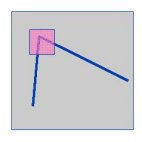
\includegraphics{images/cornerbasic}}
	\par A partir disso caímos em três casos: 
	\begin{itemize}
		\item[\Checkmark] Não há mudança em nenhuma direção.
		\item[\Checkmark] No caso de uma borda, não há mudança em uma direção.
		\item[\Checkmark] Em uma quina há mudanças significativas em todas as direções.
	\end{itemize}
	\par A função de Harris é dada por\\ 
	\par\centerline{$E(u,v) = \sum w(x,y)[I(x+u, y+v) - I(x,y)]^2$}
	%		Não há mudança em nenhuma direção.
	Onde a função de pode ser dada por:\\
	\par
	\centerline{$w(x,y) = 1$  se pertencer ao \textit{template} e}
	\centerline{$w(x, y) = 0$ caso contrário}
	\par Considerando a variação de $1px$, podemos dizer que Harris toma a variância do gradiente da imagem em uma direção, e os pontos de interesse é onde esse valor é alto.
	\par Baseado no detector de Harris, há o SURF (\textit{Speed Up Robust Detector}), que implementa o algoritmo de Harris, mas usando uma matriz Hessiana definida por
	\[ Hessian = \left| \begin{array}{ccc}
	\ L_{xx}(p, \theta) & L_{xy}(p, \theta)\\
	L_{xy}(p, \theta) & L_{yy}(p, \theta)  \\
	\end{array}\right|\]
	\par Onde L são as segundas derivadas de um ponto em uma direção em uma imagem em escala de cinza.
	O ponto de interesse é definido então e é aplicado um filtro de vizinhança ao redor do mesmo para que possamos definir a região de interesse desse objeto. Feito isso, basta procurar os pontos semelhantes na imagem do objeto.
	\section{Metodologia}
	\paragraph{}
		O código desenvolvido em C++ usando Opencv tem a parte do algoritmo de Harris (Resultado apresentado abaixo) e a parte de correspondência de pontos em seguida a qual foi feita usando SURF e um \textit{matcher} baseado em Flann. Como sugerido na documentação da biblioteca. O código não está otimizado e apresenta-se extremamente lento. Primeiro, deve-se preencher o frame da câmera com o objeto desejado e clicar na janela, para que se possa capturar a imagem do objeto, logo após essa etapa o programa detecta os pontos de interesse e mapeia o objeto no vídeo baseado nos melhores pontos e desenhando uma linha ao redor dele. É importante frisar que o SURF é invariante à rotação do objeto. 
		Para avançar da detecção de Harris para a comparação por SURF basta dar 'esc' na primeira janela.
	\section{Resultados}
	\paragraph{}
		Os resultados obtidos para cada etapa do objeto são apresentados a seguir.
		
		\par Para o algoritmo de Harris, conseguimos o seguinte resultado:
		
		\centerline{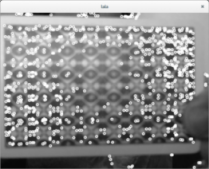
\includegraphics{images/1}}
		\centerline{\textit{resultado da detecção de Harris}}\par
		\centerline{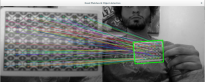
\includegraphics{images/teste}}
		\centerline{\textit{resultado de SURF}}\par
		\centerline{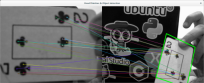
\includegraphics{images/rotacao}}
		\centerline{\textit{Objeto rotacionado}}
	\section{Conclusão}
	\paragraph{}
		Pode-se observar a grande quantidade de pontos de interesse extraídos de uma imagem bem detalhada pelo método de Harris, mas por haver o valor da distancia dos pontos de interesse e da região ao redor, é mais interessante um algoritmo mais robusto como SURF para comparação entre o objeto e a imagem, pode-se ver também que não há problema em ocluir parte do objeto ou rotacioná-lo nem mesmo mudar a escala altera a detecção, assim, temos um ótimo método para identificação de um objeto conhecido em um contexto qualquer
	\section{Bibliografia}
	\paragraph{} LAGANIÈRE, Robert, 2011. OpenCV 2 Computer Vision Application
	Programming Cookbook 
	\par COLLINS, Robert. Lecture 06:
	Harris Corner Detector. Disponível em:\\
	\url{http://www.cse.psu.edu/~rtc12/CSE486/lecture06.pdf}
	
	
	
	
\end{document}